\documentclass[aspectratio=169]{beamer}
% Beamer presentation for MNIST project
\usetheme{Madrid}

% Required packages
\usepackage{tikz}
\usepackage{pgfplots}
\usepackage{booktabs}
\usepackage{amsmath,amssymb}
\usepackage{graphicx}

% TikZ/PGF setup
\usetikzlibrary{arrows.meta,positioning,shapes.geometric}
\pgfplotsset{compat=1.18}

% Metadata
\title{MNIST-Klassifikation mit einem Fully Connected Neural Network}
\subtitle{Projektpr\'esentation}
\author{Vades Ngounouo Djoko \\ Lister Melaguie}
\institute{Cours: Deep Learning}
\date{\today}

\begin{document}

% ============================================================
% FOLIE 1: TITEL
% ============================================================
\begin{frame}
  \titlepage
\end{frame}

% ============================================================
% FOLIE 2: EINLEITUNG
% ============================================================
\begin{frame}{Einleitung}
  \begin{itemize}
    \item Ziel: Klassifikation handgeschriebener Ziffern (0--9) mit hoher Genauigkeit.
    \item Modelltyp: Mehrschichtiges Fully Connected Neural Network (MLP).
    \item Fokus:
    \begin{itemize}
      \item effizientes Training mit \textbf{SGD + Momentum},
      \item robuste Generalisierung durch \textbf{Early Stopping},
      \item nachvollziehbare Auswertung mit Metriken und Konfusionsmatrix.
    \end{itemize}
    \item Ergebnis: Testgenauigkeit von ca. \textbf{98\%}.
  \end{itemize}

  % Placeholder:
  % Insert a project overview screenshot here later.
\end{frame}

% ============================================================
% FOLIE 3: DATENSATZ
% ============================================================
\begin{frame}{Datensatz: MNIST}
  \begin{columns}[T]
    \column{0.58\textwidth}
      \begin{itemize}
        \item 70{,}000 Graustufenbilder handgeschriebener Ziffern.
        \item Bildgro\ss e: \(28 \times 28\) Pixel.
        \item Eingabevektor nach Flattening: \(28 \cdot 28 = 784\) Merkmale.
        \item 10 Klassen: Ziffern 0 bis 9.
      \end{itemize}

      \vspace{0.3cm}
      \textbf{Preprocessing}
      \begin{itemize}
        \item Normalisierung der Pixelwerte auf \([0,1]\).
        \item Umformung: Bild \(\rightarrow\) 1D-Featurevektor.
      \end{itemize}

    \column{0.42\textwidth}
      \begin{figure}
        \centering
        % Placeholder area for MNIST image grid
        \fbox{\rule{0pt}{3.8cm}\rule{0.95\linewidth}{0pt}}
        \caption{MNIST-Beispielbilder (Platzhalter)}
      \end{figure}
      % Placeholder:
      % Replace this box with your dataset screenshot.
  \end{columns}
\end{frame}

% ============================================================
% FOLIE 4: ARCHITEKTUR (MIT DIAGRAMM)
% ============================================================
\begin{frame}{Modellarchitektur}
  \begin{columns}[T]
    \column{0.5\textwidth}
      \begin{itemize}
        \item Feedforward-Netz:
        \[
          784 \rightarrow 128 \rightarrow 64 \rightarrow 10
        \]
        \item Aktivierung (hidden): ReLU
        \item Output: Logits (f\"ur CrossEntropyLoss)
      \end{itemize}

      \vspace{0.2cm}
      \small
      \textbf{Intuition:}
      \begin{itemize}
        \item Layer 1 lernt grundlegende Strichmuster.
        \item Layer 2 verdichtet zu ziffernspezifischen Merkmalen.
        \item Output-Layer ordnet Wahrscheinlichkeiten den 10 Klassen zu.
      \end{itemize}

    \column{0.5\textwidth}
      \centering
      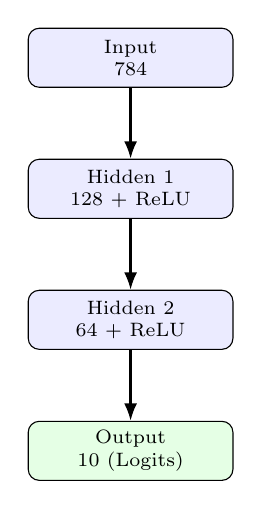
\begin{tikzpicture}[
        node distance=0.9cm,
        every node/.style={font=\scriptsize},
        layer/.style={draw, rounded corners, minimum width=2.6cm, minimum height=0.75cm, align=center, fill=blue!8},
        >={Latex[length=2.2mm]}
      ]
        \node[layer] (in) {Input\\784};
        \node[layer, below=of in] (h1) {Hidden 1\\128 + ReLU};
        \node[layer, below=of h1] (h2) {Hidden 2\\64 + ReLU};
        \node[layer, below=of h2, fill=green!10] (out) {Output\\10 (Logits)};

        \draw[->, thick] (in) -- (h1);
        \draw[->, thick] (h1) -- (h2);
        \draw[->, thick] (h2) -- (out);
      \end{tikzpicture}

      % Placeholder:
      % Optional: replace this diagram by a notebook screenshot.
  \end{columns}
\end{frame}

% ============================================================
% FOLIE 5: PARAMETER-TABELLE
% ============================================================
\begin{frame}{Parameter und Hyperparameter}
  \small
  \begin{table}
    \centering
    \begin{tabular}{@{}ll@{}}
      \toprule
      \textbf{Komponente} & \textbf{Wert} \\
      \midrule
      Architektur & \(784 \rightarrow 128 \rightarrow 64 \rightarrow 10\) \\
      Trainierbare Parameter & \(\approx 107\,\text{K}\) \\
      Optimizer & SGD + Momentum (\(0.9\)) \\
      Lernrate & \(0.01\) \\
      Loss-Funktion & CrossEntropyLoss \\
      Batch-Gr\"o\ss e & \(64\) \\
      Early Stopping & Geduld \(= 3\) \\
      Zielgenauigkeit & \(\sim 98\%\) \\
      \bottomrule
    \end{tabular}
  \end{table}

  % Placeholder:
  % Add a screenshot of your training config/logs here.
\end{frame}

% ============================================================
% FOLIE 6: TRAINING
% ============================================================
\begin{frame}{Training-Setup}
  \begin{itemize}
    \item Mini-Batch-Training mit Batch-Gr\"o\ss e \(64\).
    \item Optimierung per SGD mit Momentum:
    \[
      v_t = 0.9\,v_{t-1} + \eta \nabla_{\theta}\mathcal{L}(\theta),
      \quad \theta \leftarrow \theta - v_t,
      \quad \eta=0.01
    \]
    \item Verlustfunktion:
    \[
      \mathcal{L} = \text{CrossEntropyLoss}(\hat{y}, y)
    \]
    \item Early Stopping mit Geduld \(3\):
    Training stoppt, wenn sich die Validierungsleistung 3 Epochen nicht verbessert.
  \end{itemize}

  % Placeholder:
  % Insert screenshot of your training loop output.
\end{frame}

% ============================================================
% FOLIE 7: ERGEBNISSE (MIT DIAGRAMMEN)
% ============================================================
\begin{frame}{Ergebnisse: Lernkurven und Genauigkeit}
  \begin{columns}[T]
    \column{0.56\textwidth}
      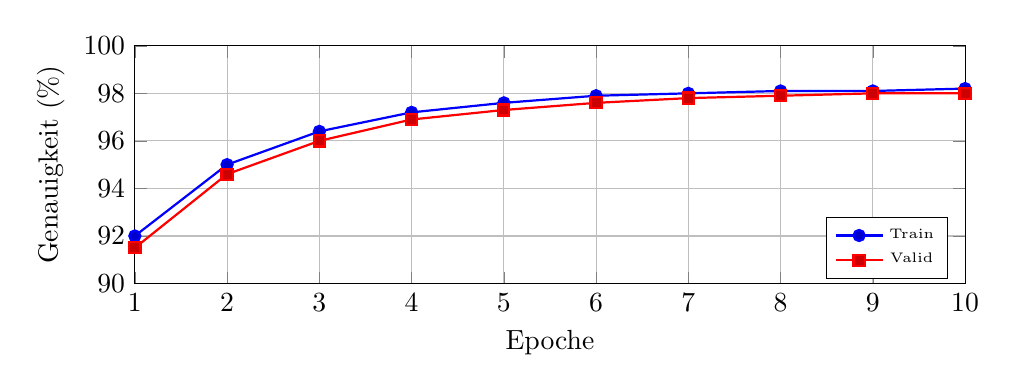
\begin{tikzpicture}
        \begin{axis}[
          width=\linewidth,
          height=4.6cm,
          xlabel={Epoche},
          ylabel={Genauigkeit (\%)},
          xmin=1, xmax=10,
          ymin=90, ymax=100,
          grid=both,
          legend style={font=\tiny, at={(0.98,0.02)}, anchor=south east}
        ]
          % Placeholder values
          \addplot+[mark=*, thick] coordinates {
            (1,92.0) (2,95.0) (3,96.4) (4,97.2) (5,97.6)
            (6,97.9) (7,98.0) (8,98.1) (9,98.1) (10,98.2)
          };
          \addlegendentry{Train}

          \addplot+[mark=square*, thick] coordinates {
            (1,91.5) (2,94.6) (3,96.0) (4,96.9) (5,97.3)
            (6,97.6) (7,97.8) (8,97.9) (9,98.0) (10,98.0)
          };
          \addlegendentry{Valid}
        \end{axis}
      \end{tikzpicture}

    \column{0.44\textwidth}
      \begin{block}{Kernaussagen}
        \begin{itemize}
          \item Stabile Konvergenz ab fr\"uhen Epochen.
          \item Kein starkes Overfitting sichtbar.
          \item Testgenauigkeit: \textbf{ca. 98\%}.
        \end{itemize}
      \end{block}

      \vspace{0.2cm}
      % Placeholder:
      % Optionally add extra chart (loss, precision/recall).
  \end{columns}
\end{frame}

% ============================================================
% FOLIE 8: KONFUSIONSMATRIX
% ============================================================
\begin{frame}{Konfusionsmatrix}
  \centering
  \begin{tikzpicture}
    \begin{axis}[
      width=10.5cm,
      height=6.3cm,
      view={0}{90},
      colormap/viridis,
      colorbar,
      xlabel={Vorhergesagte Klasse},
      ylabel={Wahre Klasse},
      xmin=-0.5, xmax=9.5,
      ymin=-0.5, ymax=9.5,
      xtick={0,1,2,3,4,5,6,7,8,9},
      ytick={0,1,2,3,4,5,6,7,8,9},
      enlargelimits=false,
      point meta min=0,
      point meta max=100
    ]
      % Synthetic placeholder values
      \addplot[matrix plot*, mesh/rows=10, point meta=explicit] table[meta=C] {
        x y C
        0 0 99  1 0 0  2 0 0  3 0 0  4 0 0  5 0 0  6 0 1  7 0 0  8 0 0  9 0 0
        0 1 0   1 1 99 2 1 0  3 1 0  4 1 0  5 1 0  6 1 0  7 1 1  8 1 0  9 1 0
        0 2 0   1 2 0  2 2 98 3 2 1  4 2 0  5 2 0  6 2 0  7 2 1  8 2 0  9 2 0
        0 3 0   1 3 0  2 3 1  3 3 97 4 3 0  5 3 1  6 3 0  7 3 0  8 3 1  9 3 0
        0 4 0   1 4 0  2 4 0  3 4 0  4 4 98 5 4 0  6 4 0  7 4 0  8 4 0  9 4 2
        0 5 0   1 5 0  2 5 0  3 5 1  4 5 0  5 5 97 6 5 1  7 5 0  8 5 1  9 5 0
        0 6 1   1 6 0  2 6 0  3 6 0  4 6 0  5 6 1  6 6 98 7 6 0  8 6 0  9 6 0
        0 7 0   1 7 1  2 7 1  3 7 0  4 7 0  5 7 0  6 7 0  7 7 98 8 7 0  9 7 0
        0 8 0   1 8 0  2 8 0  3 8 1  4 8 0  5 8 1  6 8 0  7 8 0  8 8 98 9 8 0
        0 9 0   1 9 0  2 9 0  3 9 0  4 9 2  5 9 0  6 9 0  7 9 0  8 9 0  9 9 98
      };
    \end{axis}
  \end{tikzpicture}

  % Placeholder:
  % Replace with your real confusion matrix values or image.
\end{frame}

% ============================================================
% FOLIE 9: ERKENNTNISSE
% ============================================================
\begin{frame}{Erkenntnisse}
  \begin{itemize}
    \item Ein kompaktes MLP erreicht auf MNIST bereits sehr starke Leistung (\(\sim98\%\)).
    \item SGD mit Momentum liefert stabile und gut interpretierbare Trainingsdynamik.
    \item Early Stopping (Geduld 3) reduziert unn\"otige Epochen und sch\"utzt vor Overfitting.
    \item H\"aufige Fehlklassifikationen treten zwischen visuell \"ahnlichen Ziffern auf
    (z.B. 4/9, 3/5, 7/1).
  \end{itemize}

  % Placeholder:
  % Add misclassified image examples here.
\end{frame}

% ============================================================
% FOLIE 10: VERBESSERUNGEN
% ============================================================
\begin{frame}{M\"ogliche Verbesserungen}
  \begin{itemize}
    \item Wechsel auf CNN-Architektur (Convolution + Pooling) f\"ur bessere r\"aumliche Merkmalsextraktion.
    \item Regularisierung erg\"anzen:
    \begin{itemize}
      \item Dropout,
      \item Weight Decay,
      \item Lernraten-Scheduler.
    \end{itemize}
    \item Systematische Hyperparameter-Suche (z.B. lr, Hidden-Dimensionen, Batch-Gr\"o\ss e).
    \item Datenaugmentation f\"ur robustere Generalisierung.
  \end{itemize}

  % Placeholder:
  % Add "Current vs Next Experiment" screenshot/table.
\end{frame}

% ============================================================
% FOLIE 11: FAZIT
% ============================================================
\begin{frame}{Fazit}
  \begin{block}{Zusammenfassung}
    Das Modell mit Architektur \(784 \rightarrow 128 \rightarrow 64 \rightarrow 10\)
    und ca. \(107\,\text{K}\) Parametern erreicht mit
    \textbf{SGD (Momentum 0.9), lr=0.01, CrossEntropyLoss, Batch 64}
    und \textbf{Early Stopping (Geduld 3)} eine Genauigkeit von rund \textbf{98\%}.
  \end{block}

  \vspace{0.3cm}
  \begin{itemize}
    \item Ziel erreicht: hohe Genauigkeit bei \"uberschaubarer Modellkomplexit\"at.
    \item N\"achster Schritt: CNN-basierte Variante f\"ur potenziell weitere Verbesserung.
  \end{itemize}

  \vspace{0.5cm}
  \centering
  \Large Vielen Dank!
\end{frame}

\end{document}
